\def \imgpath {"./figures/colls"}
\section{Collisions of heavy nuclei}

\subsection{Collision geometry, Centrality, multiplicity}

Collisions of heavy nuclei, composed of many fluctuating nucleons, may occur under various initial state configurations. Some quantities used to describe them are the impact parameter $b$, defined as the distance between the two nuclei centers, number of participating (scattered) nucleons $\Npart$, and the number of binary nucleonic collisions $\Ncoll$.

Determining these quantities is important because:
\begin{enumerate}
\item Soft processes, such as light flavor particle production, are expected to scale with the interaction volume, which $\propto \Npart$.
\item Hard processes, such as jet and heavy flavor production, are expected to scale with the number of large momentum transfer interactions given by \Ncoll.
\item $b$, disregarding the fluctuations of nucleonic positions, defines the shape and anisotropy of the overlap region, which are important initial state conditions.
\end{enumerate}

Since these quantities cannot be directly measured, they need to be modelled. The charged particle \textit{multiplicity} is commonly used for this purpose, as \meanNch increases monotonically with \Npart, \Ncoll, and decreasing $b$. Multiplicity \Nch can be measured experimentally, e.g.\ with tracking detectors. The concept of \textit{centrality} is also used, which is defined as quantiles of the total nuclear cross-section. For example, a centrality of $0-5\%$ refers to low $b$ values and the top $5\%$ of \Nch values (central events), while $95-100\%$ centrality refers to high $b$ values and the bottom $5\%$ of \Nch values (peripheral events). Centrality can also be inferred from other \textit{event activity} classifiers, such as amplitudes of scintillators at forward rapidity, transverse energy in calorimeters, or energy from beam remnants in zero-degree-calorimeters.

In AA collisions, these relationships are well-defined, and thus the models perform well. The most popular model is the MC Glauber model. Other models include MC-KLN and IP Glasma.

\begin{figure}[H]
\subfloat[][]{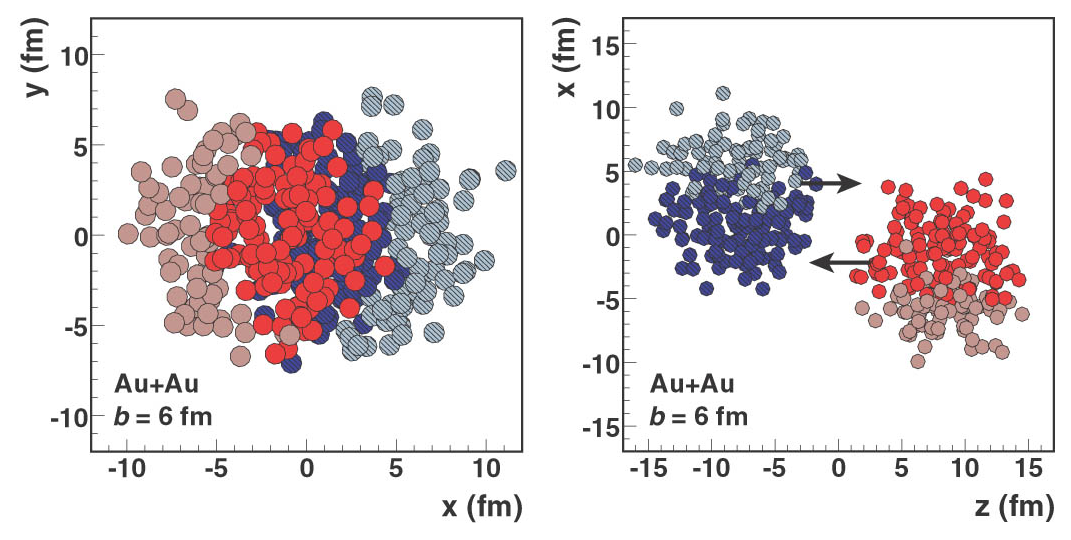
\includegraphics[width=.660\textwidth]{\imgpath/glauber_mc_event.eps}}\\
\subfloat[][]{\includegraphics[width=.660\textwidth]{\imgpath/cocktail3.eps}}
\caption{TBA}
\label{fig:colls:centrality}
\end{figure}

\subsection{MC Glauber model}

The MC Glauber model takes on a very simple albeit powerful approach. The two nuclei are simulated in three dimensions in a way that satisfies their respective nuclear density profiles, usually modelled by sampling the positions of nucleons from the Wood-Saxon distribution:

\begin{minipage}{0.5\linewidth}
    \begin{center}
        \begin{tikzpicture}
            \draw[->] (-0.25,0) -- (2.5,0) node[right] {$r$};
            \draw[->] (0,-0.2) -- (0,1.2) node[above] {$n(r)$};
            \draw[scale=1,domain=-0.15:2.2,smooth,variable=\x,blue] plot ({\x},{1/(1+exp((\x-1.5)/0.1))});
            \draw[dashed] (1.5,0) node[below] {$R$} -- (1.5,1);
        \end{tikzpicture}
    \end{center}
\end{minipage}%
\begin{minipage}{0.5\linewidth}
    \begin{equation}
        n(r) = \frac{1}{1+\exp((r-R)/a)} \quad ,
    \end{equation}
\end{minipage}

where $R$ is the nuclear radius and $a$ the nuclear skin thickness.

The nucleonic densities can be represented by uniform disks, or more accurately by Fermi-distributions or Gaussian profiles to account for fluctuations of their densities. Their parameters are left free and are tuned to the data.

A random impact parameter is then chosen or sampled. The collision is then treated as a sequence of independent binary nucleon-nucleon collisions, where
\begin{enumerate}
\item nucleons remain travelling in straight lines,
\item the inelastic nucleon-nucleon cross section $\sigma_\mathrm{NN}$ does not depend on the number of interactions,
\item two nucleons are considered to interact if their transverse relative distance $d \leq \sqrt{\sigma_\mathrm{NN}/\pi}$.
\end{enumerate}

Fig.~\ref{fig:colls:centrality} illustrates an example of a Glauber Monte Carlo event for a Au+Au collision. By simulating numerous collisions, the average \Npart and \Ncoll are determined\footnote{It also shows the scaling between the numbers of participants and binary collisions, which is approximately $\Ncoll \approx 0.35 \Npart^{4/3}$ .}, and their relations to centrality and event activity observables are determined by fitting to experimental data.

Recent studies have extended the MC Glauber model to include sub-nucleonic structures. Such efforts show that the production of charged hadrons at mid-rapidity scales linearly with the number of participating partons. Comparisons with LHC data at \snnt{5.02} suggest that the number of sub-nucleonic degrees of freedom ranges from $3$ to $5$ \cite{loizides-extendedMC}.

\section{Quark-gluon plasma}

In agreement with lattice QCD predictions, the QGP has been measured in ultra-relativistic collisions of heavy nuclei at RHIC \cite{rhic-qgp}, LHC \cite{lhc-qgp}, and even SPS \cite{sps-qgp}. Although it cannot be observed directly, a wealth of evidence from three decades of research combining various observables reveals the effects of the produced QGP medium. Whilst somewhat context-dependent, the following features make QGP the most extreme phenomena observed phenomena in terms of its:
\begin{itemize}
\item \textit{Temperature}: QGP temperatures reach values on the order of hundreds of MeV, which corresponds to approximately $2 \times 10^{12}$~K.\footnote{Contrasting some of the lowest temperatures required for the super-conducting magnets of the LHC, $T \approx 1.9$~K.}
\item \textit{Viscosity}: the shear viscosity to entropy density ratio $\eta/s$ reaches the minimum quantum limits of $1/4\pi$, making it an almost perfect liquid.
\item \textit{Vorticity}: in semi-peripheral collisions, the rotating plasma reaches a vorticity parameter of approximately $0.4$ fm$^{-1}$.
\item \textit{Magnetic field}: in non-central collisions, the magnetic fields of the heavy nuclei may peak at $\sim 10^{19}$ T.
\end{itemize}

\begin{figure}[H]
\includegraphics[width=.90\textwidth]{\imgpath/evolution.jpg}\\
\caption{TBA}
\label{fig:colls:evolution}
\end{figure}

Figure~\ref{fig:colls:evolution} illustrates the mainstream paradigm of a heavy nuclei collisions evolution:
\begin{enumerate}
\item The Lorentz-contracted heavy nuclei approach each other at ultra-relativistic speeds.
\item \textit{Pre-hydrodynamisation stage} ($\tau \equiv \sqrt{t^2 - z^2} \leq 1$ fm/c): ``hard" particles are produced in scatterings with the highest momentum transfer $Q^2$, produced matter expands rapidly in longitudinal directions and starts expanding in radial direction.
\item \textit{Hydrodynamisation} ($1 \leq \tau \leq 10$ fm/c): partons are abundantly produced, creating a deconfining medium and allowing the system to be described by hydrodynamic equations.
\item \textit{Chemical freeze-out} ($\tau \sim 20$ fm/c): the cools down, hadronises, produced hadrons then stop interacting inelastically and the system's chemical content is stabilised.
\item \textit{Thermal freeze-out}: hadrons no longer interact elastically and their kinematics stabilize.
\end{enumerate}

The following subsections outline some of the essential phenomena related to the production of QGP.

\subsection{Quarkonium dissociation and sequential suppression}

Heavy quarkonia are vector mesons of $c\bar{c}$ and $b\bar{b}$. They include $J/\psi$, $\psi(2\mathrm{S})$, $\Upsilon(1\mathrm{S})$, $\Upsilon(2\mathrm{S})$, $\Upsilon(3\mathrm{S})$, which can be relatively easily measured in LHC experiments via their di-lepton decay channels. They are created solely in the first phases of the collision and then experience the entire evolution of the QGP medium:
\begin{equation}
t^{Q\overline{Q}}_\mathrm{creation} < t^\mathrm{QGP}_\mathrm{creation} < t^\mathrm{QGP}_\mathrm{lifetime} \ll t^{Q\overline{Q}}_\mathrm{lifetime} \quad .
\end{equation}

Additionally, due to their large binding energies, their radii may remain smaller than the plasma screening radius $r_\mathrm{D}(T)$, and thus, survive the dissociation. For instance, considering their in-vacuum radii determined from the $q\bar{q}$ potential, $r_{\Upsilon(1\mathrm{S})}\sim 0.14$~fm, $r_{\Upsilon(2\mathrm{S})}\sim 0.28$~fm, $r_{\Upsilon(3\mathrm{S})}\sim 0.39$~fm, which contrast the $r_\pi \sim 0.7$~fm. This implies that different temperatures result in the dissociation of different states, and measuring the production of different states can help infer QGP temperature, as illustrated in Fig.~\ref{fig:colls:thermometer}.

\begin{figure}[H]
\includegraphics[width=.70\textwidth]{\imgpath/spec.eps}
\caption{TBA}
\label{fig:colls:thermometer}
\end{figure}

The production of heavy quarkonia in AA collisions is compared to that in pp collisions through the nuclear modification factor, $R_{\mathrm{AA}}$. This factor is widely used in various other AA measurements and is defined as:
\begin{align}
R_{\mathrm{AA}}=\frac{\mathrm{d}N_{\mathrm{AA}}/\mathrm{d}\pt}{\langle N_{\mathrm{coll}}\rangle\ \mathrm{d}N_{\mathrm{pp}}/\mathrm{d}\pt} \quad .
\end{align}
$R_{\mathrm{AA}}$ can take on the following values:
\begin{enumerate}
\item $R_\mathrm{AA} = 1$: There is no net effect on the production, corresponding to the absence of the QGP medium and other nuclear effects.
\item $R_\mathrm{AA} < 1$: The production is overall suppressed, for example, due to dissociation.
\item $R_\mathrm{AA} > 1$: The plasma and nuclear effects systematically enhance the measured production.
\end{enumerate}

At LHC energies, the abundance of charm quarks in the QGP is high enough that charmonia can be reformed after dissociation, which somewhat complicates the interpretation of their suppression. However, the $\Upsilon(3\mathrm{S})$ bottomonium has $R_{\mathrm{AA}}$ consistent with 0 at $\sqrt{s_{\mathrm{NN}}}=5.02$ TeV, as shown in Figure \ref{fig:colls:cmsupsilon}. This complete suppression is a clear signature of the QGP and can be used together with models to estimate the QGP temperature at these energies as $T\approx 630$~MeV.

\begin{figure}[H]
\subfloat[][]{\includegraphics[width=.40\textwidth]{\imgpath/cms_ups1.pdf}} 
\subfloat[][]{\includegraphics[width=.39\textwidth]{\imgpath/cms_ups2.pdf}}
\caption{TBA}
\label{fig:colls:cmsupsilon}
\end{figure}

\subsection{Strangeness enhancement}

TBA

\subsection{Collective flow}

TBA

\subsection{Jet quenching}

TBA

\subsection{Cold nuclear matter effects}

It should be noted that apart from the QGP, other effects come into play due to the fact that the collision involves two nuclei instead of two protons. These effects are important caveats to bear in mind and include:

\begin{enumerate}
\item Nuclear (anti-)shadowing: Reflects the modification in production due to differences in nPDFs and PDFs.
\item Cronin effect: Describes the initial parton energy loss due to scatterings in the nuclear medium and broadens measured \pt spectra.
\item Nuclear absorption: Describes the dissociation of particles due to their interactions with the passing-by nuclear remnants. It is generally negligible at LHC energies.
\item Co-mover absorption: This is the effect of inelastic interactions with the hadron gas.
\end{enumerate}

These effects can be isolated and quantified in pA or very peripheral AA collisions.

\section{QGP phenomena in small systems}

Measurements within the last decade have shown that certain QGP phenomena can also be observed in high-multiplicity events of pp collisions at LHC energies, which challenges the traditional assumption that QGP is only produced in AA collisions. This has sparked debates about the existence of QGP in pp collisions and, to a lesser degree, about the absence of QGP in AA collisions, despite the extensive experimental evidence.

Furthermore, the observed behavior of these phenomena indicates that the role of event multiplicity \Nch may be more significant than system size. This has led to ongoing efforts to establish a consistent and seamless link between the paradigms of pp and AA collisions.

\subsubsection{Strangeness and charm enhancement}

ALICE measurements on $\LA/\pi$, $\XI/\pi$, and $\Omega/\pi$ ratios demonstrate that the production rates of particles containing strange quarks increase faster with multiplicity than those containing only u and d quarks. This also depends on the strangeness content -- the effect is the strongest for $\Omega$ and vanishes for protons. Furthermore, the evolution to larger systems seems to be continuous with respect to \Nch. The measurements can be seen in Fig.~\ref{fig:colls:ssstrangeness}.

To contrast the strangeness measurements with heavier flavour, the $J/\psi \ /\pi$ ratio also shows a clear increase in yield with increasing \Nch in pp collisions, as is shown in Fig.~\ref{fig:colls:ssstrangeness}. However, this comes with an important caveat: high-multiplicity events are biased to have enhanced hard processes, as discussed further in Chapter X. Moreover, the evolution of this phenomenon is also not continuous with \Nch when going from pp collisions at \sppt{13} to \snnt{5.02}, which can also be explained by the fact that charm quarks are produced solely in hard scattering processes, the rates of which depend on the collision system and center-of-mass energy.

\begin{figure}[H]
\subfloat[][]{\adjincludegraphics[trim={0 0 {.48\width} 0},clip,height=15em]{\imgpath/ss_strangeness1.pdf}}\hspace{2em}
\subfloat[][]{\adjincludegraphics[trim={0 0 {.948\width} 0},clip,height=15em]{\imgpath/ss_strangeness2.pdf}\adjincludegraphics[trim={{.52\width} 0 0 0},clip,height=15em]{\imgpath/ss_strangeness2.pdf}} 
\caption{TBA}
\label{fig:colls:ssstrangeness}
\end{figure}

\subsubsection{Anisotropic flow}

Azimuthal correlations and anisotropic flow measurements in small collision systems exhibit features similar to those observed in AA collisions, hinting at the presence of collective expansion. However, in small systems, these measurements are particularly challenging due to their large sensitivity to non-flow effects, such as jet fragmentation or resonance decays, which can mimic the features of collective flow. 

While models using hydrodynamic-like descriptions seem to be able to describe the data, especially at high multiplicities, the interpretation of the results in small systems is still under investigation. The values of elliptic flow $v_2$ seem to be comparable to those in low-multiplicity Pb-Pb collisions, although the evolution of $v_2$ across different system sizes does not appear to be smooth. The measurements from CMS displaying a clear ridge in high-multiplicity events and the $v_2$ results from ALICE can be seen in Fig.~\ref{fig:colls:ssv2}.

\begin{figure}[H]
\subfloat[][]{\adjincludegraphics[trim={0 {0.67\height} 0 0},clip,width=0.45\textwidth]{\imgpath/ss_ridge1.pdf}}
\subfloat[][]{\adjincludegraphics[trim={0 {0.67\height} 0 0},clip,width=0.45\textwidth]{\imgpath/ss_ridge2.pdf}}\\
\adjincludegraphics[trim={0 {0.7\height} 0 0},clip,width=0.8\textwidth]{\imgpath/ss_v2.pdf}
\subfloat[][]{\adjincludegraphics[trim={0 0 0 {0.967\height}},clip,width=0.8\textwidth]{\imgpath/ss_v2.pdf}}
\caption{TBA}
\label{fig:colls:ssv2}
\end{figure}

\subsubsection{Radial flow}

Measurements of the ratio of \LA to \KOs \pt spectra ratio were also studied in pp collisions with differing \Nch. The boost of a collectively expanding system, as expected in the context of radial flow, should have a greater impact on heavier hadrons, leading to an enhancement of the baryon-to-meson ratio at intermediate \pt. This enhancement is observed in the \ltok ratio, its magnitude increases with increasing \Nch and the peak position shifts towards higher values collisions, consistent with the hydrodynamic picture. The increase at intermediate momenta leads to a corresponding depletion at low \pt. Integrated (or high-\pt) \ltok ratios exhibit essentially no (or minor) multiplicity dependence. This observation also applies to proton-to-pion ratios. 

Recent studies have also investigated the charmed baryon-to-meson ratio $\LA_c/\mathrm{D^0}$, with similar findings, although measurements with smaller uncertainties are still required. Fig.~\ref{fig:colls:ssrflow} presents the corresponding results.

\begin{figure}[H]
\includegraphics[width=.90\textwidth]{\imgpath/ss_rflow.pdf}
\caption{TBA}
\label{fig:colls:ssrflow}
\end{figure}

\subsubsection{Sequential suppression of $\Upsilon$ states}

While defining $R_\mathrm{AA}$ to compare high-multiplicity and low-multiplicity events is unclear, and measuring yields as a function of \Nch is complicated by its biases related to the hardness of primary scatterings, it is worthwhile to investigate the ratio of excited-to-ground states of quarkonia as a function of \Nch.

Interestingly, these results exhibit a decrease with increasing \Nch, resembling the pattern of sequential suppression due to QGP deconfinement. Even more remarkable, this dependence disappears in low-sphericity, jet-dominated, events (event shape observables such as sphericity are discussed in more detail in Chapter X). These findings, reported in Fig.~\ref{fig:colls:ssupsilon}, suggest that the dependence on \Nch is solely influenced by the UE, rather than jets. As event multiplicity grows larger, excited $\Upsilon$ states become relatively less likely to be measured compared to the ground state.

These results indicate the need for a better understanding of $\Upsilon$ hadronization and the role UE may play in it. They also raise the question of whether the ground state is enhanced rather than the excited states being suppressed. Additionally, the effects of the mass differences must also be considered. However, the fact that low-sphericity, jet-dominated events have the same ratios as high-sphericity, UE-dominated events at low \Nch argues against these ideas.

An important caveat to note is that hadronic decays (which are dominant) of the heavy $\Upsilon$ states may result in tens of produced \Nch. Therefore, even minor discrimination against the excited states could hypothetically be correlated with a substantial but trivial increase in the accompanying \Nch. To the author's knowledge, there are currently no available phenomenological descriptions of the observed behavior, which further limits potentially groundbreaking interpretations.

\begin{figure}[H]
\subfloat[][]{\includegraphics[width=.40\textwidth]{\imgpath/ss_ups1.pdf}} 
\subfloat[][]{\includegraphics[width=.40\textwidth]{\imgpath/ss_ups2.pdf}}
\caption{TBA}
\label{fig:colls:ssupsilon}
\end{figure}

\subsubsection{Other QGP signatures}

Jet quenching

\subsection{Role of multiplicity}

The observations made above highlight the significance of studying the role of multiplicity \Nch. In contrast to AA collisions, high-multiplicity events in pp collisions do not arise from a mere increase in the amount of colliding matter, as the values of \Npart and \Ncoll are fixed:
\begin{align}
\Npart = 2 \, ,\quad \ \Ncoll = 1 \, .
\end{align} 

Additionally, due to the relatively constant initial system volume, high-\Nch pp events may exhibit energy densities that exceed the threshold for QGP formation, given that the highest \Nch values are similar to those observed in peripheral AA collisions, where QGP formation is observed.

Clearly, the picture is more complex and despite its simplicity as an event activity classifier, \Nch poses challenges when it comes to relating data to theory since it cannot be directly linked to the initial state, and multiplicities in different events may originate from entirely different processes.

To address these issues and gain a better understanding of the evolution between low and high multiplicities and the potential for QGP formation, this dissertation focuses on transverse spherocity \SOPT and underlying event activity \RT measurements. They may offer a deeper insight into the relevant degrees of freedom involved.

%One expects a trivial difference as the pT spectra are being measured at midrapidity in the same kinematic region where the midrapidity multiplicity selection is done. However, the slope of the pT spectra at high-pT indicates that the midrapidity estimator selects harder and harder subnucleonic interactions as the multiplicity increases. The ratios obtained with the forward estimator do not show a change in slope at high-pT. Still, the hard high-pT production is more enhanced than soft low-pT production in highmultiplicity collisions and vice versa in low-multiplicity collisions. This implies that the scaling with multiplicity of soft and hard processes is fundamentally different in pp compared to nucleus–nucleus collisions.

%a study with PYTHIA 8 (Monash 2013 tune) shows that the forward multiplicity estimator has the strongest correlation between the number of MPIs and the multiplicity. For this reason, the forward multiplicity slicing is used for multiplicity selection in the rest of this section unless specifically noted otherwise. As the multiplicity selection is done on charged particles, a second advantage of the forward selection is that it does not create an imbalance between charged and neutral particles at midrapidity



\section{Phenomenological models}

\subsection{Pythia}

Description of Pythia model

\subsubsection{String interactions and Ropes}

Two paragraphs
%Explain how CR mimics flow

%In PYTHIA, hadron production occurs via the incoherent break-up of colour flux tubes called ‘strings’, which exhibit constant energy density, leading to the conclusion that even high-multiplicity events wouldresult in unchanged particle ratios. As a consequence of the observation in [487], PYTHIA modelling had to resort to conceptually different physical mechanisms to reproduce experimental data, such as the inclusion of ‘colour ropes’ – colour flux tubes with increased tension that are created whenever several strings overlap prior to hadronisation in high-multiplicity pp collisions [841]. The predictions from PYTHIA with colour ropes can be seen in Fig. 81 and describe strangeness enhancement in pp collisions within a 10\% accuracy in high-multiplicity collisions. However, it is important to note that the proton-topion ratio is not correctly described in this model, which indicates that further theoretical studies are still required for a proper description of hadrochemistry.

\subsection{Epos LHC}

Description of Epos in two paragraphs

